\documentclass[12pt]{memoir}

\usepackage{titling}

% Figures and controlling packages
\usepackage{float}
\usepackage{wrapfig}

% logo for the title page
\usepackage{adjustbox}
\newcommand{\swlogo}{
  \adjustbox{valign=t}{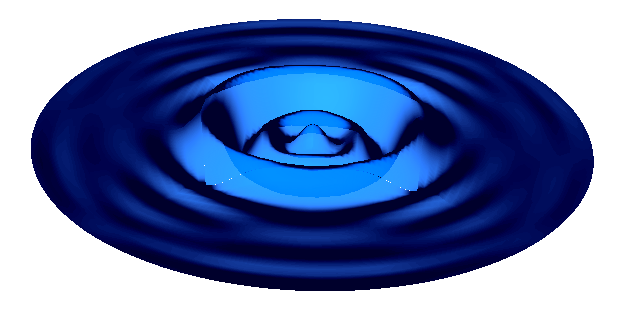
\includegraphics[width=0.25\textwidth]{images/shallowWater.png}}
}


% Adjusting the section,chapter, etc. headings
\usepackage{titlesec}
\newcommand*{\justifyheading}{\raggedleft}

\titleformat{\chapter}[display]
  {\normalfont\sffamily\huge\bfseries\justifyheading\color{blue}}
  {\chaptertitlename\ \thechapter}{20pt}{\Huge}
\titleformat{\section}
  {\normalfont\sffamily\Large\bfseries\color{cyan}}
  {\thesection}{1em}{}

\usepackage[margin=1.0in]{geometry}
\usepackage{amsmath,amsthm}
%\usepackage{breqn}
\usepackage{amsfonts}
\usepackage{amssymb}
\usepackage[mathscr]{euscript}
\usepackage{graphicx}
\usepackage{verbatim}
\usepackage[round]{natbib}
\usepackage{appendix}
\usepackage{xcolor}


% Header and Footer
\makeevenhead{myheadings}{}{}{}
\makeoddhead{myheadings}{}{}{}{}

\makeevenfoot{myheadings}{ {\fontfamily{cmss}\selectfont \theauthor} }{{\fontfamily{cmss}\selectfont schoonover.numerics@gmail.com }}{\thepage}

\makeoddfoot{myheadings}{ {\fontfamily{cmss}\selectfont \theauthor  } }{{\fontfamily{cmss}\selectfont schoonover.numerics@gmail.com} }{\thepage}

\makefootrule{myheadings}{\textwidth}{\normalrulethickness}{0ex}

\author{Joe Schoonover}
\title{Discontinuous Galerkin}
\date{}




\begin{document}
\frontmatter
% Doing a custom title-page
\begin{titlingpage}
    
        \vspace*{2cm}

   % Setup up the main and sub-titles with the logo
   {\fontfamily{cmss}\selectfont
     \begin{tabular}{l r}
           & \HUGE{\textbf{ \thetitle }}\\
           & \HUGE{\textbf{  SELF }}\\
   \swlogo & \\
           & \huge{\textbf{\textcolor{blue}{Iterative Solvers}}}
        \end{tabular}
    }    
 
        \vspace{1cm}
        

         
        \vspace{2cm}
        
     \begin{center}
     
        %Do a subtitle here if you like
        {\fontfamily{cmss}\selectfont
        \huge{
           Software Documentation
        }
        
        \vspace{1.5cm}
        
        % Enter the author's name
        \textbf{
        \large{
           \theauthor 
         }}}
        
        \vfill
        
        
     \end{center}
        
    
\end{titlingpage}


{\fontfamily{cmss}\selectfont
\tableofcontents
}
\mainmatter

% Special Style
\pagestyle{myheadings}

\chapter{Overview}
 The iterative solvers modules that are packaged with the Spectral Element Libraries in Fortran (SELF) software contain routines to perform many different types of iterative solver algorithms to compute solutions to the matrix problem
 \begin{equation}
 A \vec{x} = \vec{b}.
 \end{equation}
 The main module provides the routines for a variety of iterative solvers that rely on \textit{abstracted data structures} with only a few \textit{deferred} routines. The reason for this is to so that the module is highly reusable for many different matrix problems, and not just those that arise in the context of the SELF. A statement I have heard from colleagues while developing this object oriented set of modules is that this approach can degrade performance. If you feel this is the case, any of the routines can be copied as a template for you particular problem, and you can avoid using the interface that is described in this documentation. At the very least, you should familiarize yourself with the contents of the main module (IterativeSolvers.f90) so that you can be aware of the ``template'' algorithms that are at your disposal. For those who wish to use the interface, this documentation will describe to you 
 \begin{enumerate}
  \item the routines that \textbf{you} need to define for your problem,
  \item how to choose your iterative method,
  \item how to set up a preconditioner.
 \end{enumerate}
 
 In order to maintain generalizability, all of the routines provided store the solution and forcing in 1-D arrays. Many problems may not naturally fit with this sort of storage ( e.g. in multiple dimensions it is much more intuitive to use multi-dimensional arrays ). You are free to store your solution in any data-structure that you can imagine, so long as you can map each degree of freedom to a unique element of the 1-D array. Additionally, you will also need to define routines to map from the 1-D array back to your data structure. Aside from the book-keeping, your main goal as the programmer are to define a matrix action and a residual function. An optional (and certainly recommended) goal is to set up and define a preconditioner. Oddly enough, the preconditioner can also make use of the same iterative solvers routines but perhaps with a matrix that is quicker to invert. Of course, you can provide your own means of inverting the preconditioning matrix.
 
 
 \chapter{Verification}
 
 \section{Conjugate Gradient}
 
 \section{GMRES}
 
 \section{Method Comparisons}
 
 
\end{document}